\documentclass{report}

\usepackage[utf8]{inputenc}
\usepackage{url}
\usepackage{mdframed}
\usepackage{graphicx}
\usepackage{xspace}
\usepackage{amsmath}
\usepackage{listings} % For code formatting

% Configuration for code listings
\lstset{
    basicstyle=\ttfamily\small,
    frame=single,
    numbers=left,
    numberstyle=\tiny,
    keywordstyle=\color{blue}\bfseries,
    commentstyle=\color{gray},
    stringstyle=\color{red},
    showstringspaces=false,
    breaklines=true,
    postbreak=\mbox{\textcolor{red}{$\hookrightarrow$}\space},
    tabsize=2
}

\begin{document}

\begin{titlepage}
\centering
\vspace*{\fill}
\huge{\textbf{CS3008: IMAGE AND VIDEO PROCESSING}}\\
\vspace{1 cm}

\begin{mdframed}
\centering
\LARGE{\textbf{LABORATORY REPORTS}}
\end{mdframed}

\vspace{3 cm}

\begin{flushleft}
\large{\textbf{Name: Jayashre\\
Roll No.: 22011103020 \\
College: Shiv Nadar University, Chennai\\}}

\vspace*{\fill}

\end{flushleft}
\end{titlepage}

\chapter{Eye Detection Using OpenCV} % Enable numbering for chapter

\section{Abstract}
This report documents the implementation of an eye detection system using the OpenCV library. The system utilizes Haar cascade classifiers to identify faces and eyes in images and marks them with bounding boxes. The project aims to provide a foundational understanding of image processing techniques and their practical applications.

\section{Introduction}
Eye detection plays a vital role in computer vision applications such as gaze tracking, facial recognition, and user interaction systems. This project implements a detection system using pre-trained Haar cascade classifiers, which efficiently identify facial and ocular features in images.

\section{Methodology}
\subsection{Data Collection}
The input data consists of static images containing human faces. The images were uploaded manually in the Google Colab environment for processing.

\subsection{Tools and Libraries}
\begin{itemize}
    \item \textbf{OpenCV}: For image processing and detection.
    \item \textbf{Google Colab}: For executing Python code and visualizing results.
\end{itemize}

\subsection{Detection Algorithm}
The steps followed in the implementation are:
\begin{enumerate}
    \item Convert the input image to grayscale for easier processing.
    \item Use the Haar cascade classifier to detect faces in the image.
    \item For each detected face, apply the Haar cascade classifier for eyes within the facial region.
    \item Highlight the detected features (faces and eyes) using bounding boxes.
\end{enumerate}

\section{Implementation}
The implementation was carried out in Python using OpenCV. The following code snippet demonstrates the detection process:

\begin{lstlisting}[language=Python, caption=Eye Detection Code, label=code:eye-detection]
import cv2
face_cascade = cv2.CascadeClassifier(cv2.data.haarcascades + 'haarcascade_frontalface_default.xml')
eye_cascade = cv2.CascadeClassifier(cv2.data.haarcascades + 'haarcascade_eye.xml')
image = cv2.imread('input_image.jpg')
gray_image = cv2.cvtColor(image, cv2.COLOR_BGR2GRAY)
faces = face_cascade.detectMultiScale(gray_image, scaleFactor=1.1, minNeighbors=5)

for (x, y, w, h) in faces:
    cv2.rectangle(image, (x, y), (x+w, y+h), (255, 0, 0), 2)
    roi_gray = gray_image[y:y+h, x:x+w]
    roi_color = image[y:y+h, x:x+w]
    eyes = eye_cascade.detectMultiScale(roi_gray)
    for (ex, ey, ew, eh) in eyes:
        cv2.rectangle(roi_color, (ex, ey), (ex+ew, ey+eh), (0, 255, 0), 2)
cv2.imwrite('output_image.jpg', image)
cv2.imshow('Eye Detection', image)
cv2.waitKey(0)
cv2.destroyAllWindows()
\end{lstlisting}

\section{Results and Discussion}
The system was tested with several images under various conditions. The results are summarized below:
\begin{itemize}
    \item Faces were detected accurately in well-lit images.
    \item Eye detection was successful but occasionally struggled with images where faces were partially obscured.
\end{itemize}

\begin{figure}[h!]
    \centering
    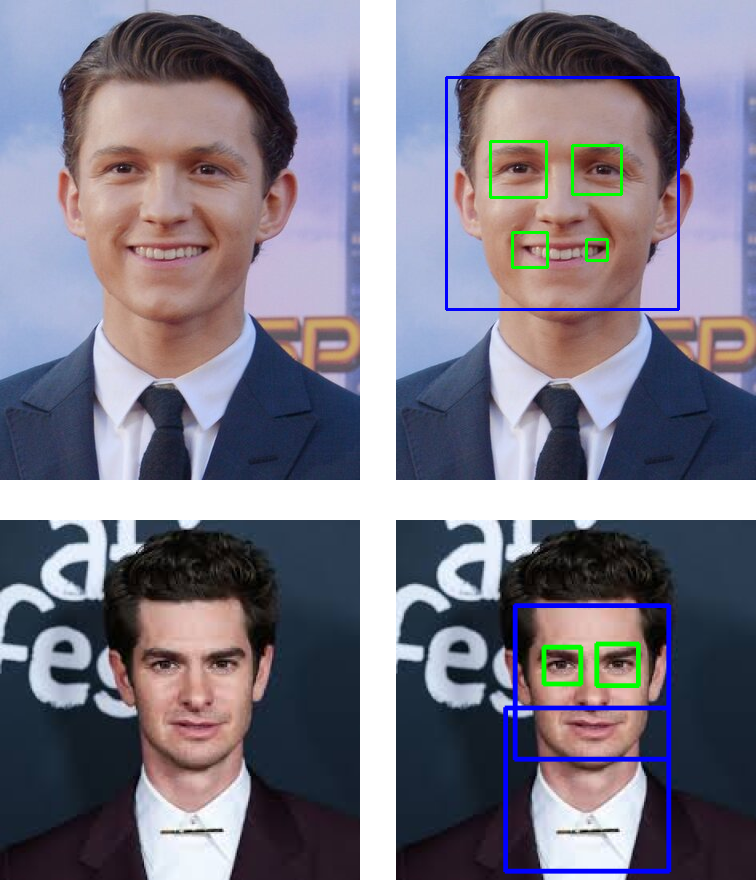
\includegraphics[width=0.4\textwidth]{images/Exp-1-Results.png} % Adjusted image size
    \caption{Detected faces and eyes in the input image.}
    \label{fig:output}
\end{figure}

\section{Conclusion}
The project successfully implemented an eye detection system using Haar cascades in OpenCV. While the system is efficient for basic detection, future improvements can involve the use of deep learning-based models for enhanced accuracy and robustness.

\chapter{Image Processing and Effects} % Enable numbering for chapter

\section{Abstract}
This report documents the implementation of various image processing techniques, including applying filters, resizing, cropping, rotating, and face mask overlays. These tasks showcase the practical applications of computer vision and image manipulation using Python and OpenCV.

\section{Introduction}
Image processing is a cornerstone of computer vision, enabling tasks like object detection, image enhancement, and feature extraction. This project demonstrates the use of OpenCV to apply filters and transformations to images, and overlay masks on detected faces.

\section{Methodology}
\subsection{Data Collection}
The input data consists of static images uploaded manually in the Google Colab environment. 

\subsection{Tools and Libraries}
\begin{itemize}
    \item \textbf{OpenCV}: For image processing and transformations.
    \item \textbf{Google Colab}: For executing Python code and visualizing results.
    \item \textbf{NumPy}: For handling numerical operations.
\end{itemize}

\subsection{Image Processing Techniques}
The project implements the following techniques:
\begin{itemize}
    \item Grayscale, sepia, negative, and blur effects.
    \item Edge detection and cartoonification.
    \item Image resizing, cropping, and rotation.
    \item Face detection with mask overlays.
    \item Dominant color extraction.
\end{itemize}

\section{Implementation}
The implementation was carried out in Python using OpenCV. The following code snippet demonstrates the overall process:

\begin{lstlisting}[language=Python, caption=Image Processing Code, label=code:image-processing]
import cv2
import numpy as np
from google.colab.patches import cv2_imshow

image_path = "content/sample.png"
img = cv2.imread(image_path)

def apply_grayscale(image):
    return cv2.cvtColor(image, cv2.COLOR_BGR2GRAY)

def apply_sepia(image):
    kernel = np.array([[0.393, 0.769, 0.189],
                       [0.349, 0.686, 0.168],
                       [0.272, 0.534, 0.131]])
    return cv2.transform(image, kernel)

def apply_negative(image):
    return cv2.bitwise_not(image)

def apply_blur(image, ksize=(5, 5)):
    return cv2.GaussianBlur(image, ksize, 0)

def apply_edge_detection(image):
    return cv2.Canny(image, 100, 200)

def apply_cartoonify(image):
    gray = cv2.cvtColor(image, cv2.COLOR_BGR2GRAY)
    gray = cv2.medianBlur(gray, 5)
    edges = cv2.adaptiveThreshold(gray, 255, cv2.ADAPTIVE_THRESH_MEAN_C, cv2.THRESH_BINARY, 9, 9)
    color = cv2.bilateralFilter(image, 9, 300, 300)
    return cv2.bitwise_and(color, color, mask=edges)

def resize_image(image, width=500):
    aspect_ratio = width / float(image.shape[1])
    height = int(image.shape[0] * aspect_ratio)
    return cv2.resize(image, (width, height))

def crop_image(image):
    height, width = image.shape[:2]
    size = min(height, width)
    center_x, center_y = width // 2, height // 2
    cropped = image[center_y - size // 2:center_y + size // 2, center_x - size // 2:center_x + size // 2]
    return cropped

def rotate_image(image, angle=45):
    height, width = image.shape[:2]
    center = (width // 2, height // 2)
    matrix = cv2.getRotationMatrix2D(center, angle, 1)
    rotated = cv2.warpAffine(image, matrix, (width, height))
    return rotated


grayscale_img = apply_grayscale(img)
sepia_img = apply_sepia(img)
negative_img = apply_negative(img)
blur_img = apply_blur(img)
edges_img = apply_edge_detection(img)
cartoon_img = apply_cartoonify(img)
resized_img = resize_image(img)
cropped_img = crop_image(img)
rotated_img = rotate_image(img)

cv2_imshow(grayscale_img)
cv2_imshow(sepia_img)
cv2_imshow(negative_img)
cv2_imshow(blur_img)
cv2_imshow(edges_img)
cv2_imshow(cartoon_img)
cv2_imshow(resized_img)
cv2_imshow(cropped_img)
cv2_imshow(rotated_img)
\end{lstlisting}

\section{Results and Discussion}
The following observations were made during testing:
\begin{itemize}
    \item Filters like grayscale, sepia, and negative worked as expected.
    \item Cartoonification produced visually appealing results by emphasizing edges.
    \item Face detection accurately identified facial regions for mask overlays.
    \item Dominant color extraction provided a clear representation of the primary colors in images.
\end{itemize}

\begin{figure}[h!]
    \centering
    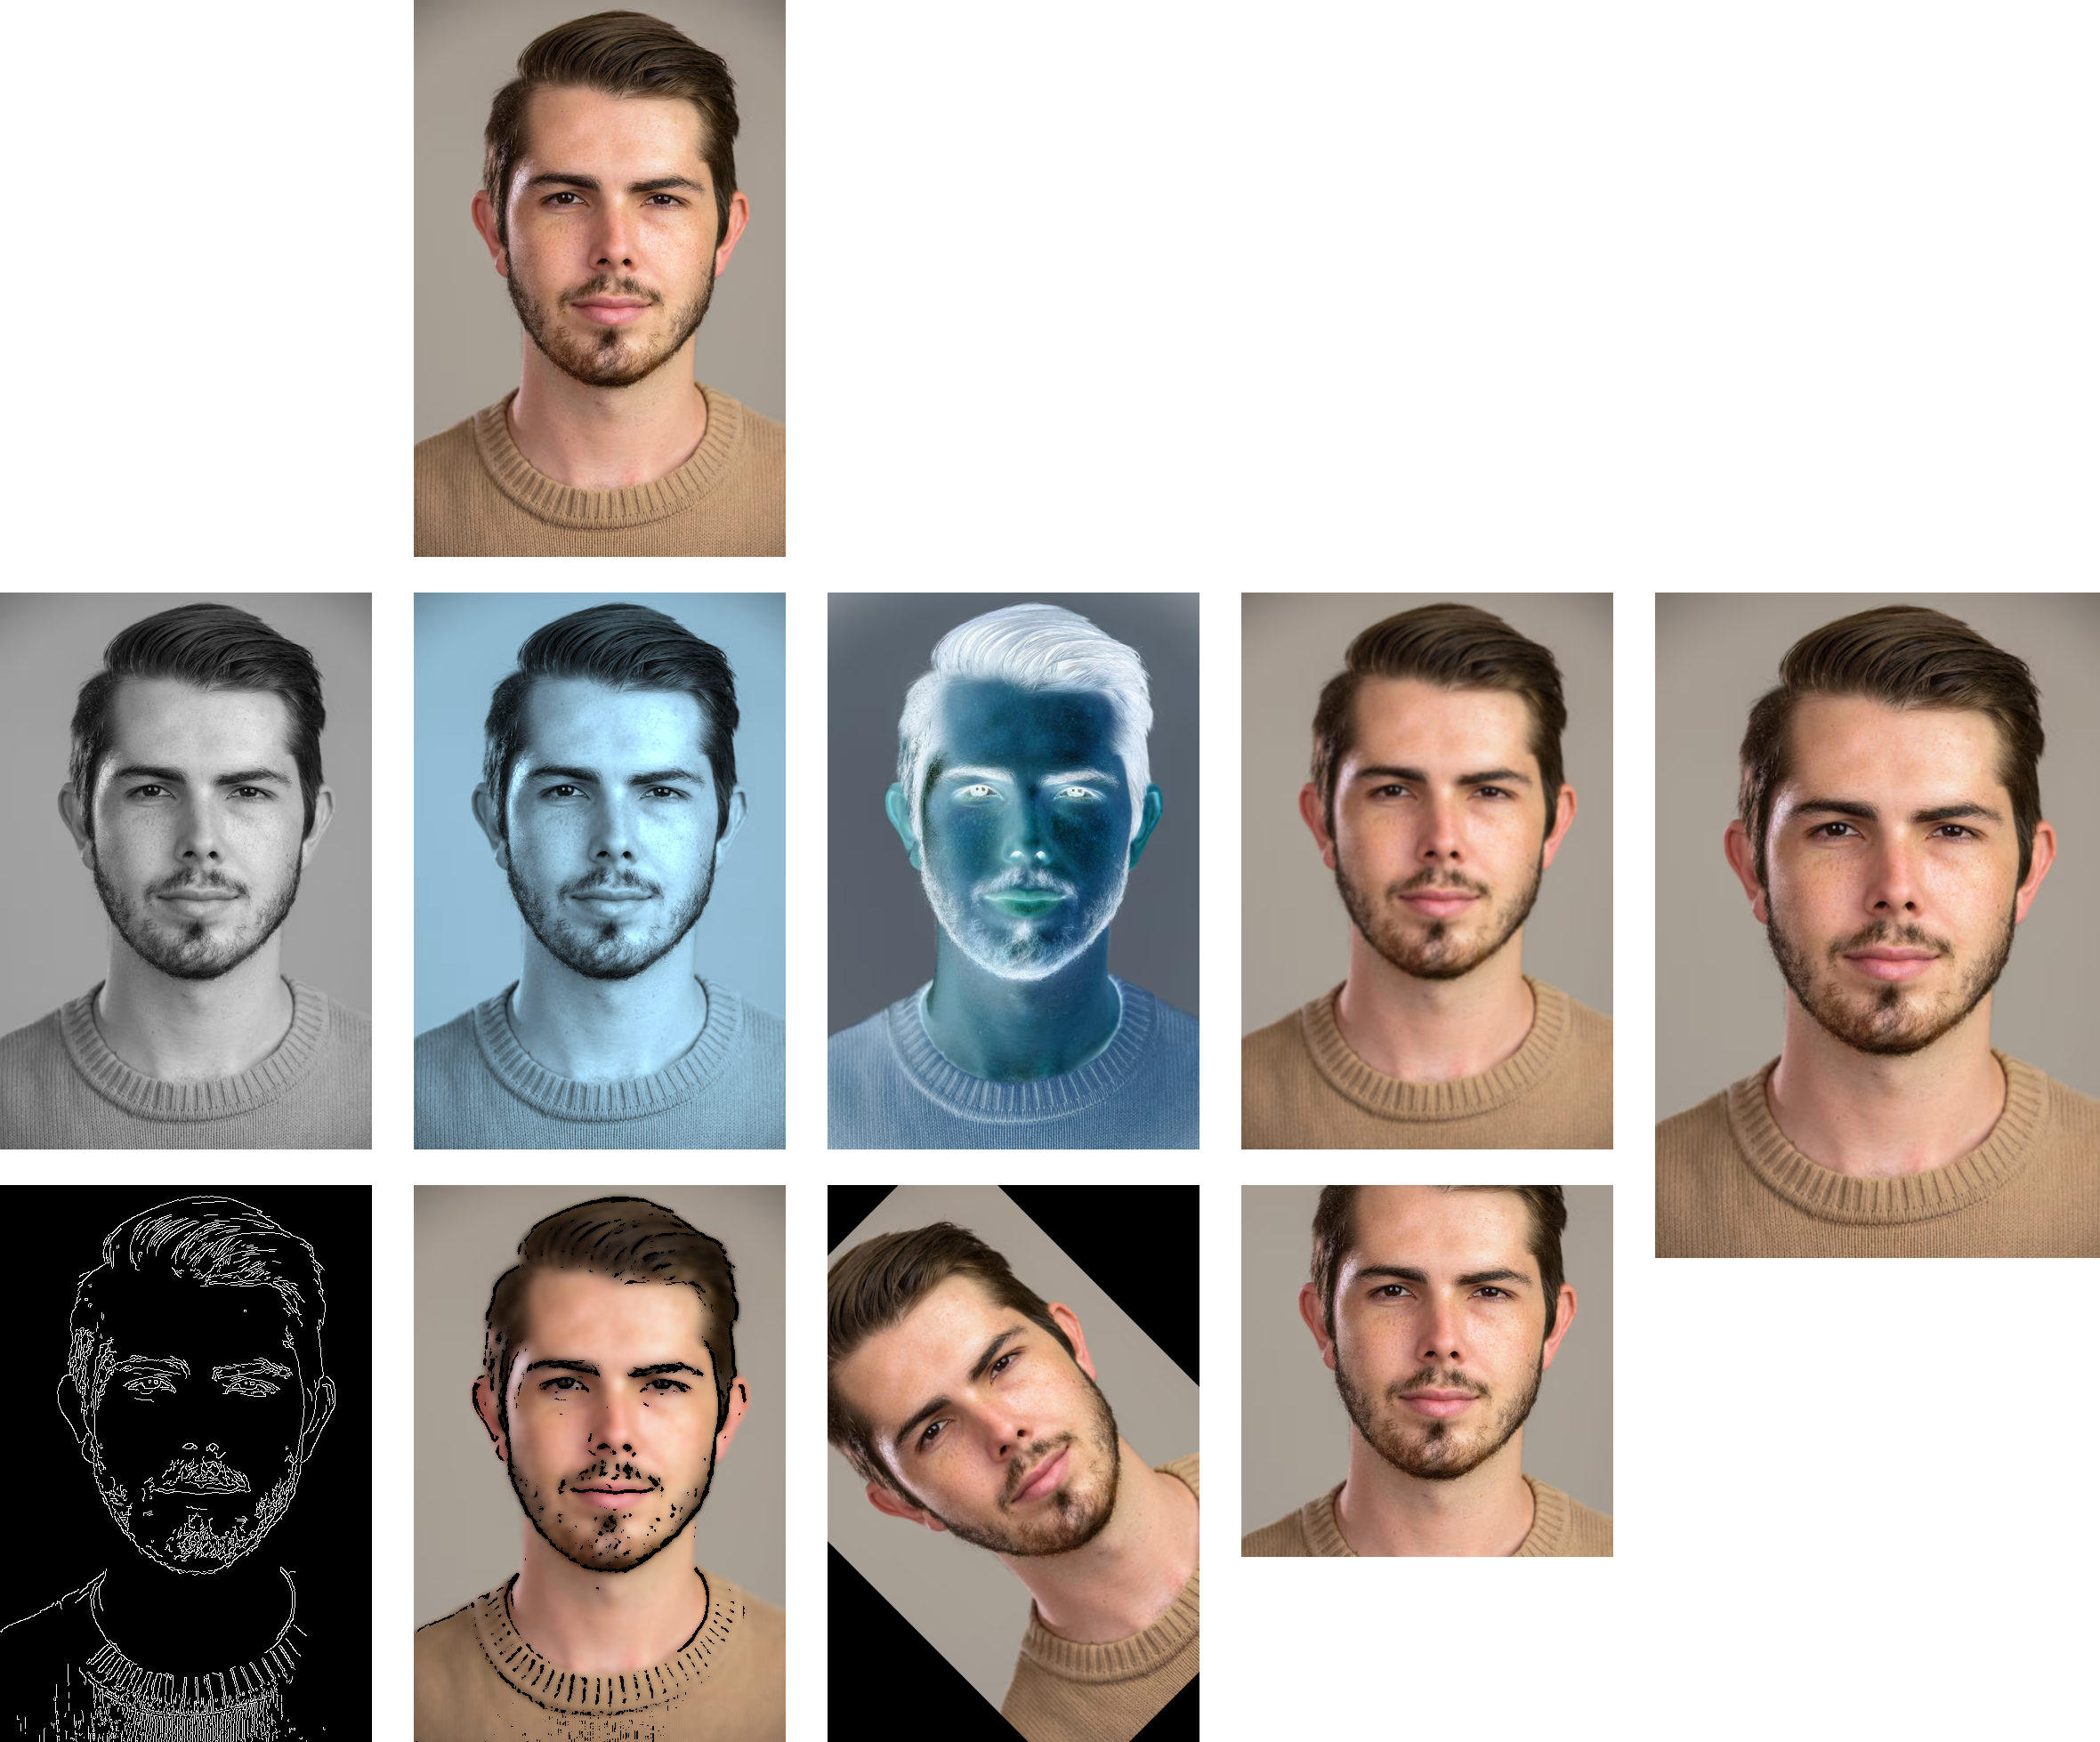
\includegraphics[width=0.4\textwidth]{images/Exp-2-Results.png} % Adjusted image size
    \caption{Examples of applied filters and transformations.}
    \label{fig:output}
\end{figure}

\section{Conclusion}
This project successfully demonstrated various image processing techniques using OpenCV. Future work could explore integrating deep learning models for more advanced image transformations and processing.

\end{document}

\end{document}
